\documentclass{article}
\usepackage[utf8]{inputenc}
\usepackage[letterpaper, portrait, margin=1in]{geometry}
% \usepackage{mathptmx}
\usepackage{fancyhdr}
\usepackage{amsmath}
\usepackage{amssymb}
\usepackage{amsfonts}
\usepackage{mathtools}
\usepackage{bm}
\usepackage{enumitem}
\usepackage{graphicx}
\usepackage{float}
% \usepackage{subfiles}
\usepackage{biblatex}
\addbibresource{bibliography.bib}


%Discrete Math commands
\renewcommand{\iff}{\leftrightarrow}
\newcommand{\T}{\text{T}}
\newcommand{\F}{\text{F}}
\newcommand{\union}{\cup}
\newcommand{\isection}{\cap}
\newcommand{\of}{\circ}

%Math commands
\renewcommand{\v}[1]{\mathbf{#1}}
\renewcommand {\inf} {\infty}
\newcommand {\cross} {\times}

%Automatic Exercise Increment Commands
\newcounter{exerciseNum}
\newcommand{\exercise}{\stepcounter{exerciseNum} \section*{Exercise \arabic{exerciseNum}}}

\pagestyle{fancy}
\fancyhf{}
\rhead{Iyer \\ Page \thepage}
\chead{SER Model\\of the Covid-19 Outbreak}


\title{SER Model of the Covid-19 Outbreak \\\large 292:H1 Final Presentation}
\author{Vibhu Iyer}
\date{\today}



\begin{document}
%setup
\maketitle

\graphicspath{{pictures/}}


{
 \centering
 \section*{Abstract}
 The SARS-CoV-2 infectious outbreak can be predicted using the SIR compartment model. Through a system of ordinary differential equations, we can model a variety of different situations and gain a better understanding of the general effects certain variables have on the spread of the disease or similar viral particles. We lay out a simplistic version of the virus and its path through a population through the differential equations that govern the SIR model, as well as consider its strengths and benefits against other models, such as simulations. Further, we will manipulate the model to better match the current data and critique the drawbacks of this slightly simplistic approach to a larger problem.
}

\tableofcontents

\section{Basic System of Equations}
We can begin by defining three groups, or ``compartments'', of subjects within a population of size $N$: $S(t)$, the number of people who have not been infected yet at time $t$, known as the \textit{susceptible} population; $I(t)$, the number of people currently infected at time $t$, known as the \textit{infected} population; and $R(t)$, the number of people who have been infected and are no longer contagious at time $t$, known as the \textit{recovered} population. From here, we can then define new variables:
$\beta$, the average number of contacts between members of the population, and $\gamma$, the rate at which the population recovers. Conceptually, if it takes $\tau$ days for a subject to pass the infection, then $1/\tau$ of the current infected population will pass on a given day, relating $\gamma = 1/\tau$. From this, we can come up with a system of ODEs:
\begin{align*}
 \frac{dS(t)}{dt}   & = -\beta I(t)S(t)/N              \\
 \frac{dI(t)}{dt}   & = \beta I(t)S(t)/N - \gamma I(t) \\
 \frac{dR(t)}{d(t)} & = \gamma I(t)
\end{align*}
To create a simulation, we begin with a very small percentage of the population being infected, with the entire population being susceptible and none of the population recovered. using the \texttt{ode45} function of MATLAB, we can numerically solve the ODE. In many cases, it is easier to deal with numbers as a percentage of the population; therefore, we if consider the population to be simply 1, or 100\%, we can set up the simulation with different starting variables. Doing so, we end up with the following solution:

\begin{figure}[H]
 \centering
 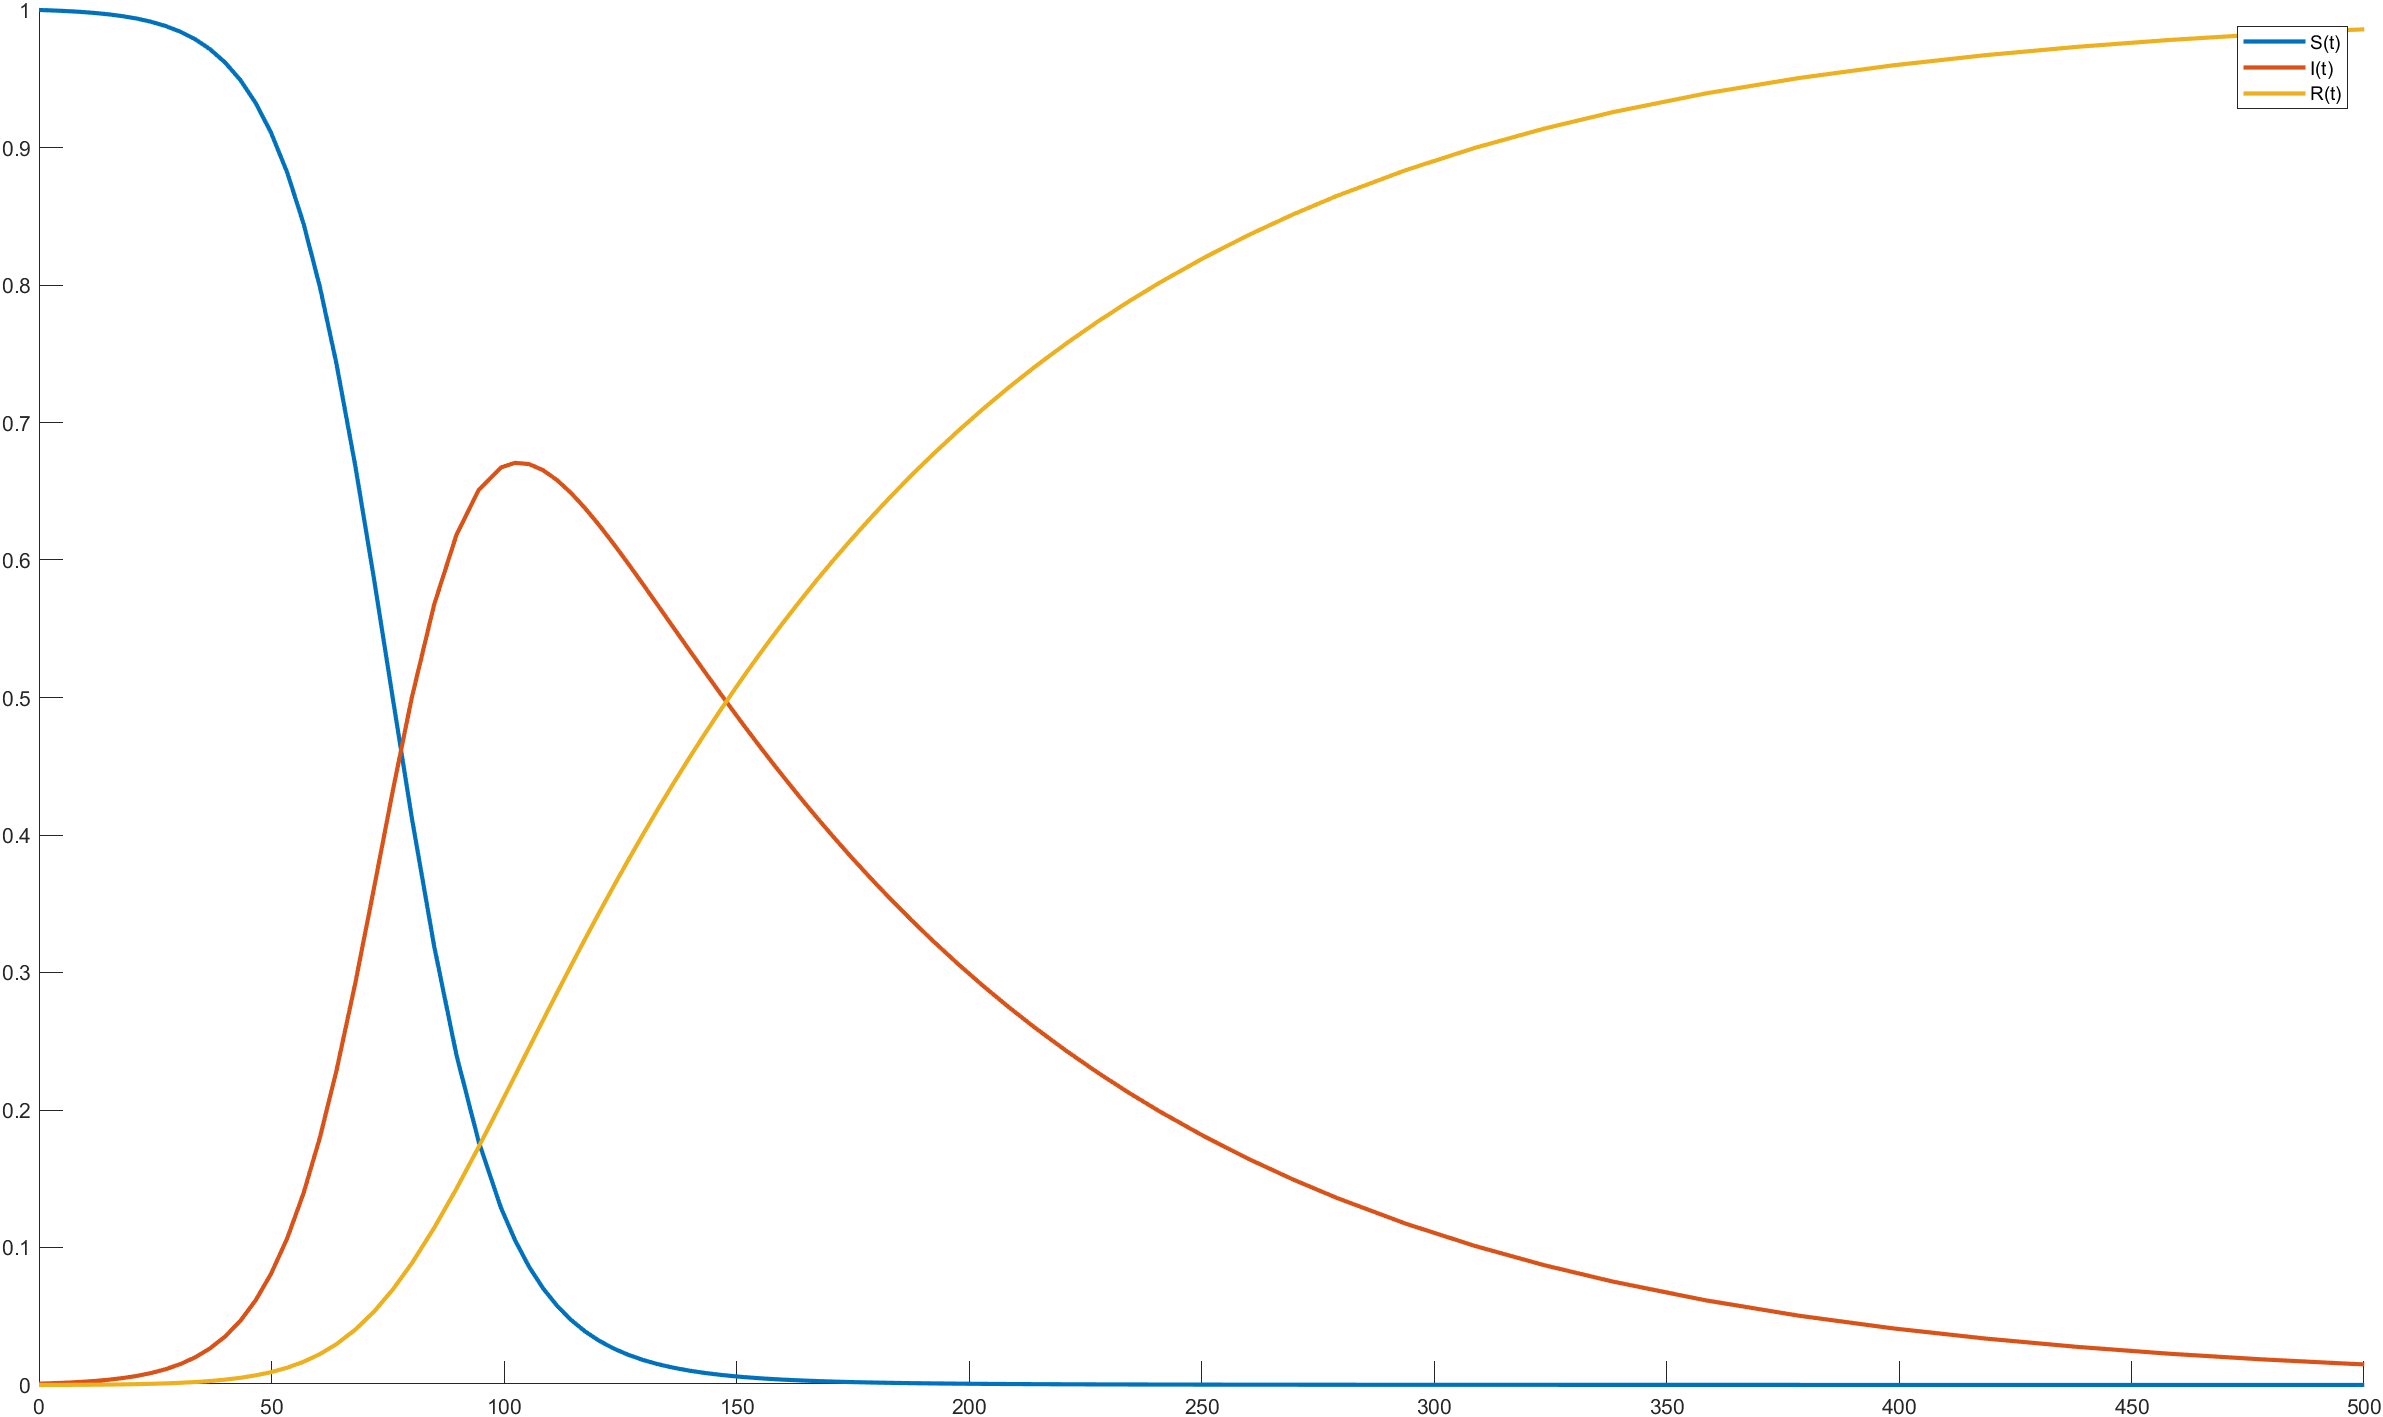
\includegraphics[scale = 0.4]{pic1.png}
 \caption{Base representation of the SIR model using ODEs}
 \label{fig1}
\end{figure}

\section{Varying Parameters}
In the numerical model, there are two main parameters that can be varied simply: $\gamma$ and $\beta$. To accurately model these parameters, we can pull from data gathered about the virus. Doing so, we get an effective mean incubation rate of 14 days. Therefore, our value of $\gamma = 1/\tau = 0.07143$. Beta, however, is slightly more complicated to estimate, as it varies per person and on a multitude of other factors (while $\gamma$ also varies, it does not vary by nearly as much as $\beta$ seems to: see \cite{rnot1}). To get a consistent value for $\beta$, it is useful to look more closely at $R_0$.

\subsection{$R_0$, the Basic Reproduction Number}
When looking at the spread of a disease, it is useful to consider how fast it spreads; one of the main ways of measuring this is the number of people a given person will spread the disease to. This is known as the effective reproduction number, $R$. However, this is incredibly difficult to track, even with contact-tracing and other modern methods of slowing a pandemic. Furthermore, this number changes as the susceptible group grows smaller over time. Instead, research focuses on a broader, more applicable number: $R_0$, the basic reproduction number. This number represents the average number of cases caused by a vector, given a base susceptible population. For COVID-19, this number ranges from 1.5-3.9 \cite{rnot2}, and for the purposes of this demonstration, we will use 2. We also have the formula $R_0 = \beta / \gamma = \beta\tau$; this can be thought of as the number of days someone will be infectious multiplied by the number of people they infect, giving the total number of people the average disease vector will infect. (Note that $R_0 > 1$ is the definition of a pandemic.) Since we know taht $\gamma = 1/14$, we have that $2 = 14\beta$, or $\beta = 0.1428$. We can then use the given numbers to create a more realistic graph of the pandemic:

\begin{figure}[H]
 \centering
 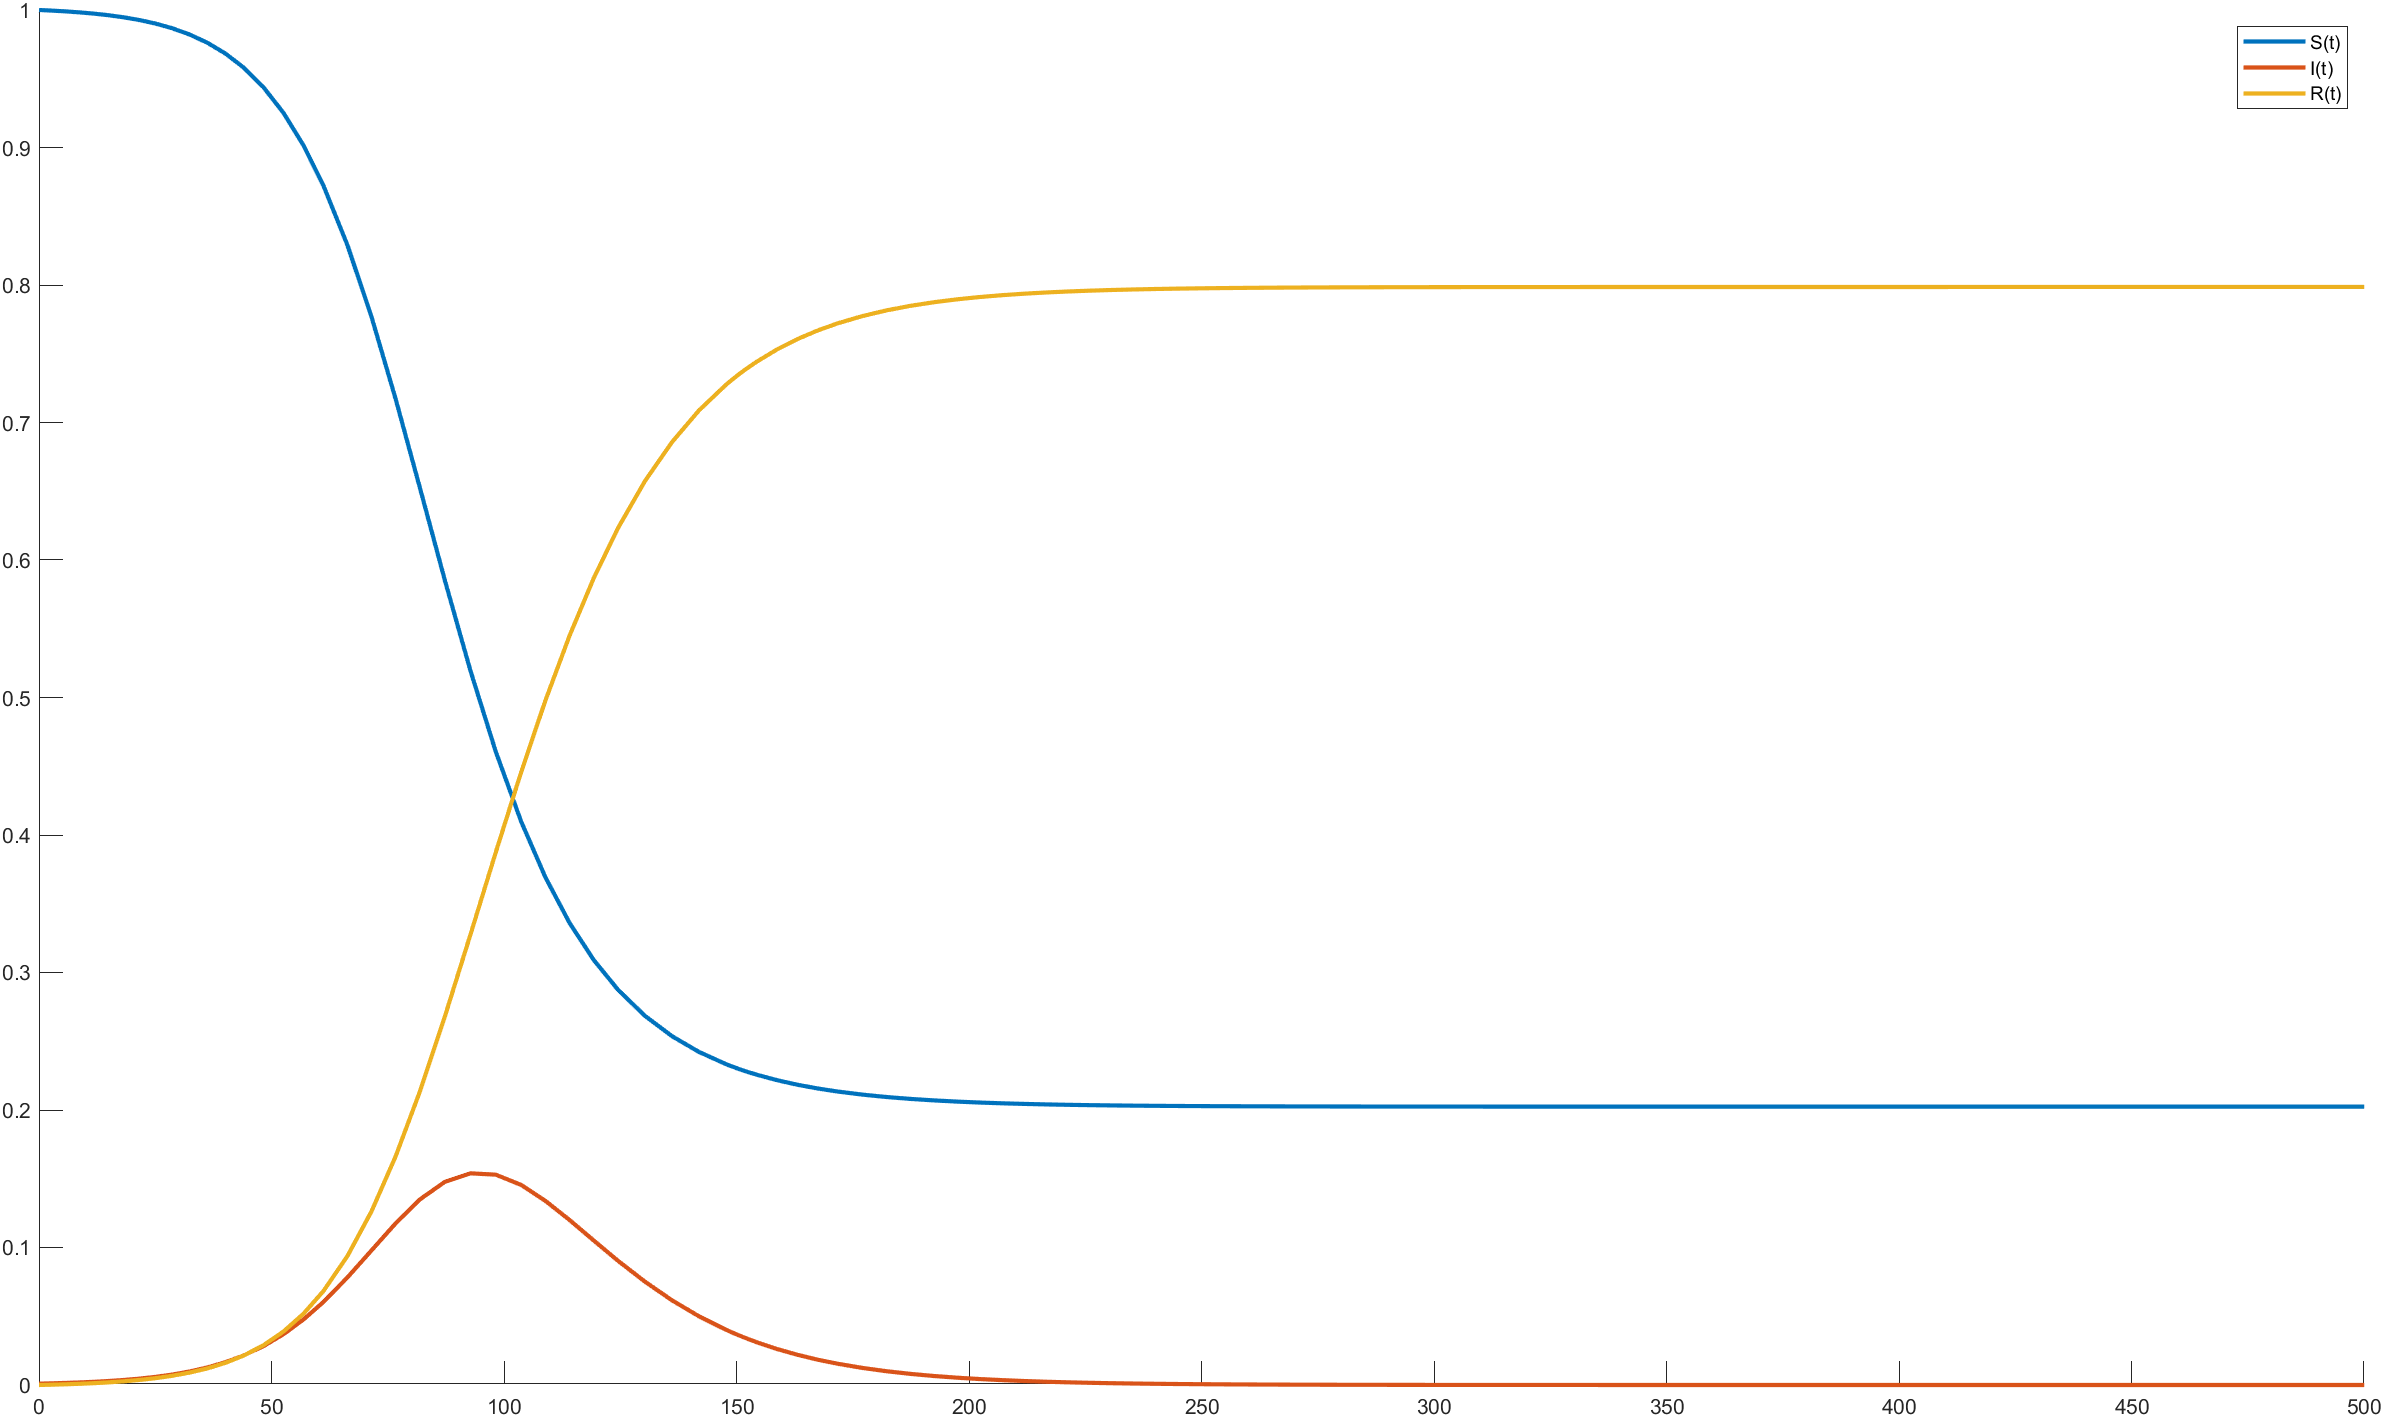
\includegraphics[scale=0.4]{pic2.png}
 \caption{$\gamma = 0.07143, \beta = 0.1428$}
 \label{fig2}
\end{figure}

Note the differences between the two pictures: the we have a much higher - and quicker - overall recovered number, which can be treated as the total number of people who have contracted the disease. Given a death rate of approximately 0.7\%, we have a death count of approximately 5\% of the population - approximately 2 million people in the U.S. alone. However, note that the peak infection occurs at approximately the same time, while the tail of the second graph is much longer; this is due to $\gamma$ being approximately the same between the two. While the disease is more ``contagious'' in the first picture, the incubation period is approximately equal for both. This also causes the entire population to contract the disease in the first example.

\section{Preventative Measures}
One of the easiest variables to add to the traditional SIR model is that of vaccination. To add a vaccinated group, we simply need to consider what vaccination does; it takes away from the susceptible groups and adds them to the removed group. For this model, we will slightly skew this, using a separate group to account for vaccinations. For the SIR ODE model, we can consider vaccinations to be somewhat based on both the time and the susceptible population; that is, as time goes on, more vaccines are handed out, but they are only handed out to the susceptible population. This helps keep the simulation under control. We can model this by changing the above equations like so"
\begin{align*}
 \frac{dS(t)}{dt} & = -\beta I(t)S(t)/N - S(t)\text{(percentvax)}max(0, \frac{(t-\text{(startDay)})}{400})/N \\
 \frac{dV(t)}{dt} & = S(t)\text{(percentvax)}max(0, \frac{(t-\text{(startDay)})}{400})/N
\end{align*}

where \texttt{percentvax} is the percentage of the susceptible population that gets the vaccine each day, and \texttt{startDay} is the day that the vaccines begine to start going out. the \texttt{max} function here serves to make the vaccination rate 0 at the beginning, and only increase when the rate is above 0.
We now have one more graph: $V(t)$, the vaccinations among the population. (Note that as $V^\prime(t)$ is also dependent on $t$, the rate of vaccination increases over time, somewhat accounting for another variable). This lends the following graph structure:


\begin{figure}[H]
    \centering
    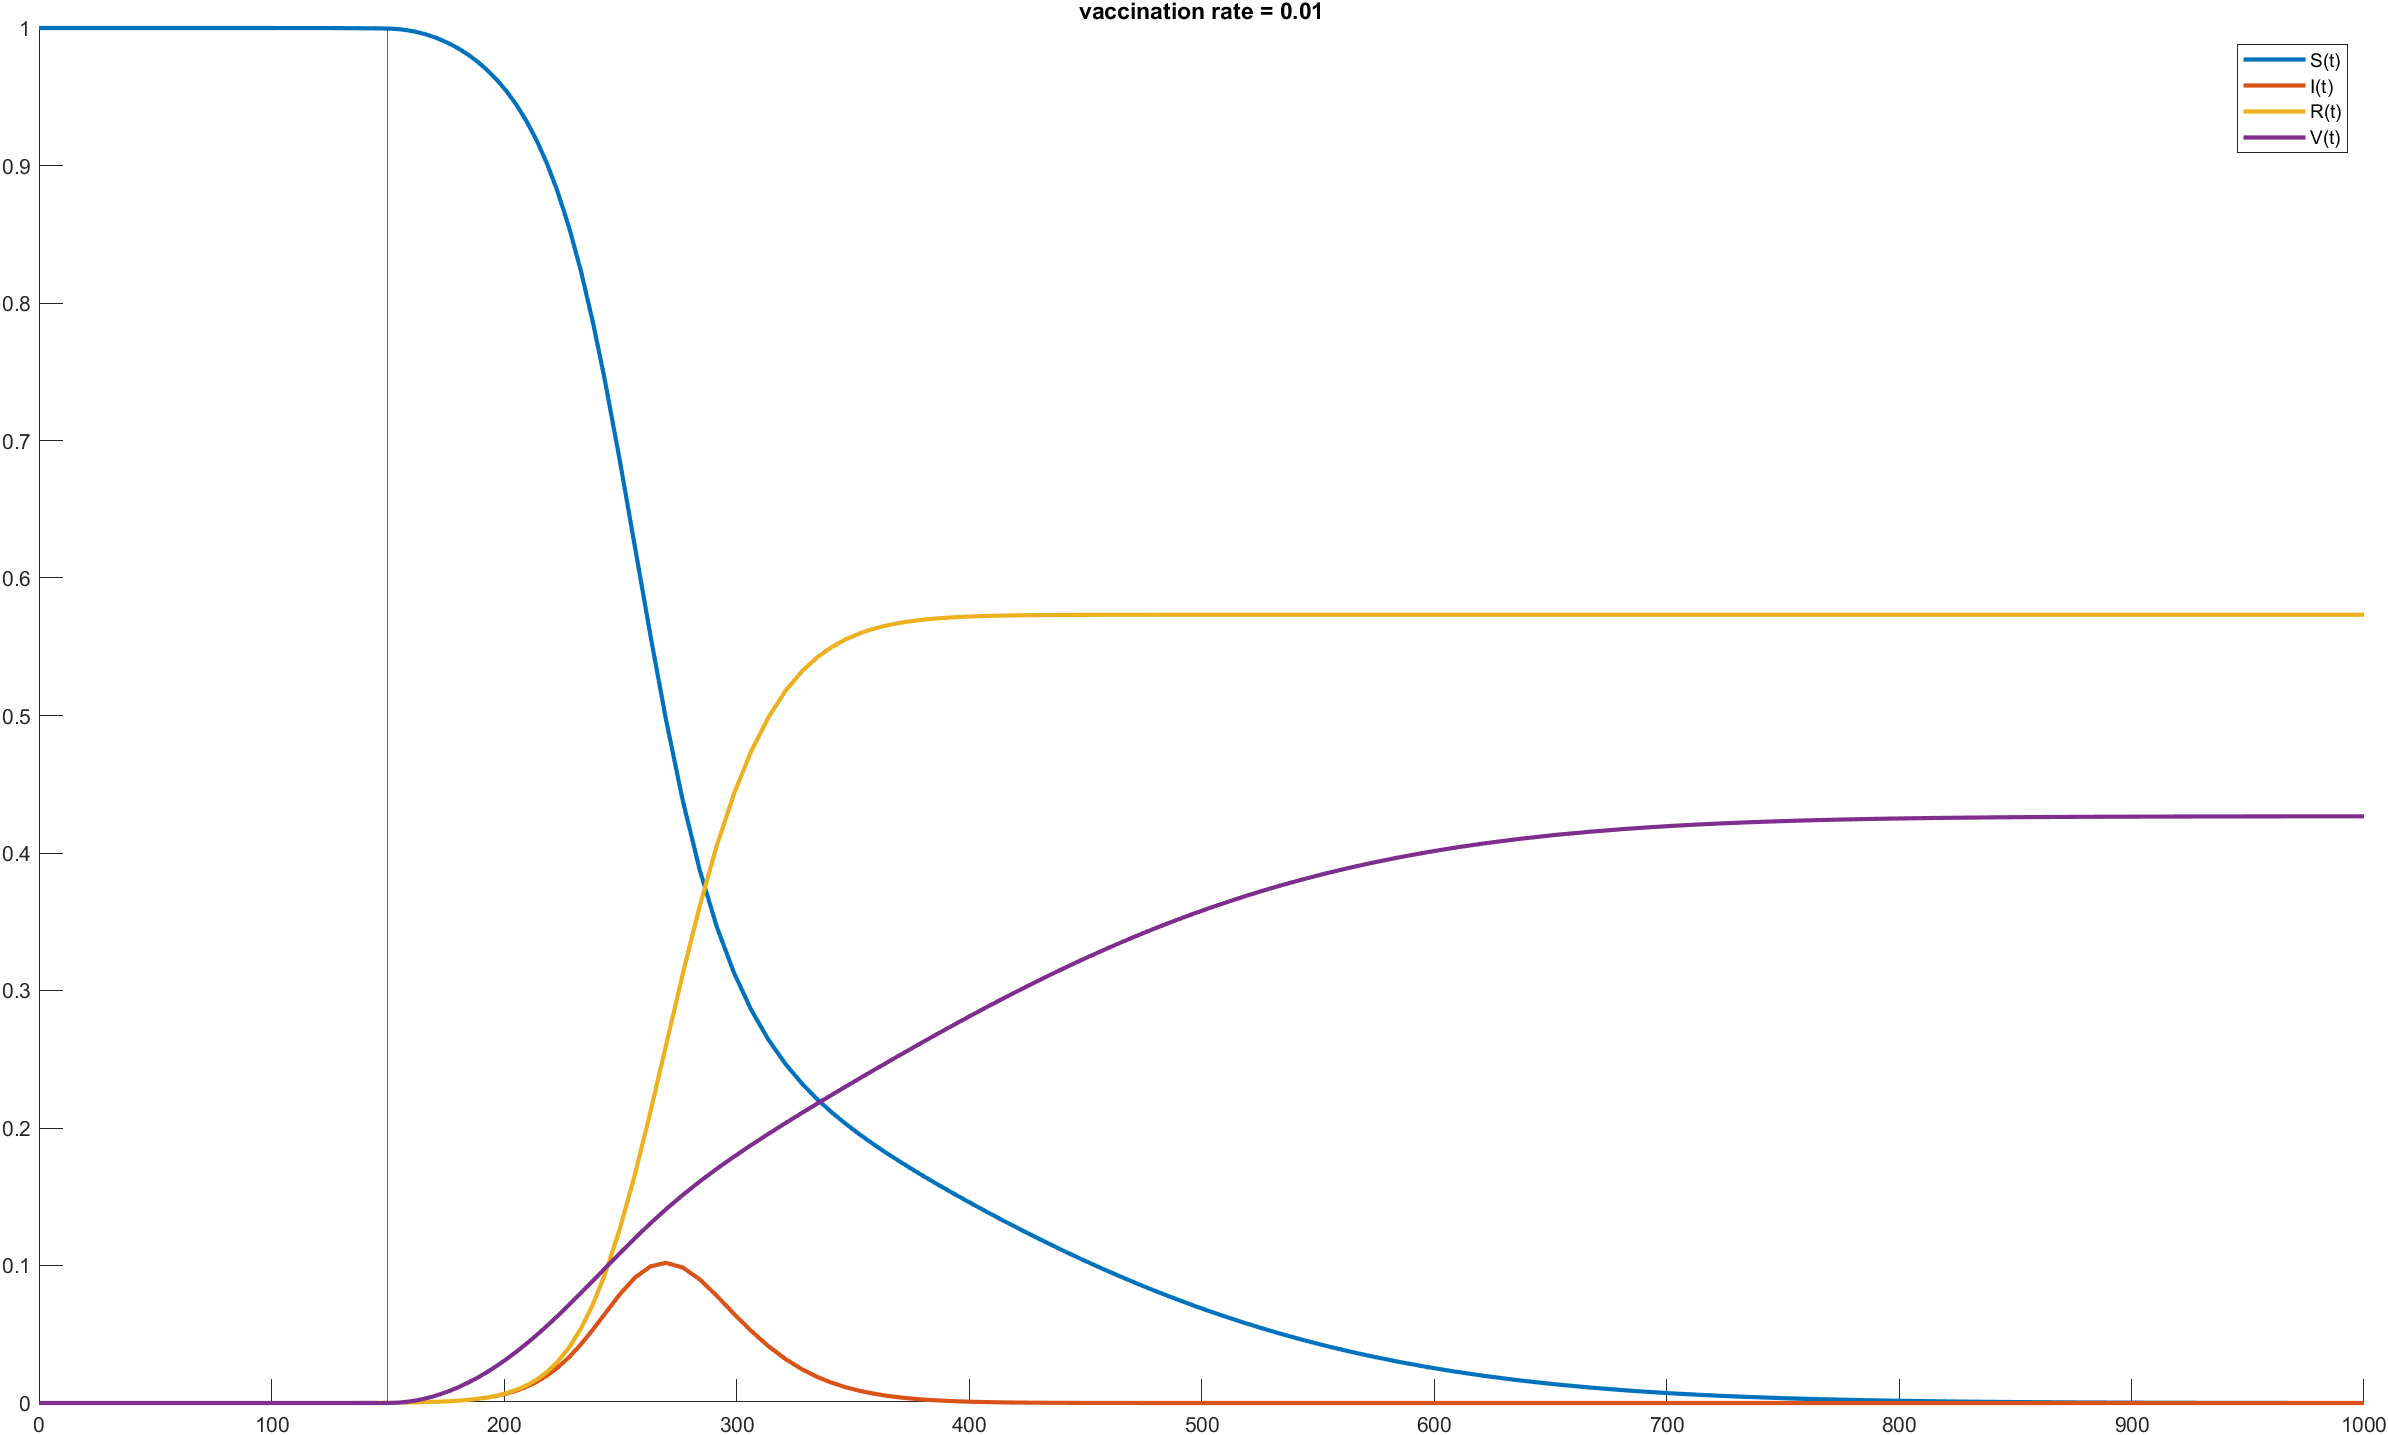
\includegraphics[scale=0.4]{vax1.png}
    \caption{Vaccination Among the Population: rate = 1\%}
    \label{fig3}
\end{figure}

The vertial line represents start day of vaccinations; see that if it is too late, the peak remains in approximately the same spot, just lower and with a smaller tail, reducing the total cases.


\section{Improvements on the Model}
There are several improvements that can be made to the SIR model; for example, it is fairly elementary to make the model have a temporary immunity period, or with a changing population based on death rate and birth date. There is also a class of models based on the SIR system known as the age-influenced model. However, all such models are subject to the Law of Large Numbers, and therefore cannot truly introduce randomness or variability into the system. In such cases, it is best to look at a simulation. While running such simulations multiple times will result in similar systems, simulations allow for a larger set of rules that can better encompass the system as a whole. For example, we can program a simulation using the following set of rules:
\begin{itemize}
    \item Let a year be 200 days. The last third of a year will have higher infection rates than the first two thirds.
    \item Each person has varying chances of being infected by their neighbors; the infection rate and incubation period vary by a deviation from the mean. For this simulation, we use the same means as above, but the infection rates vary by proximity to "hubs" within the simulation, with higher infection rates at those locations.
    \item vaccination rate increases slowly, and only susceptible individuals can be vaccinated.
    \item Most individuals follow social distancing, and therefore they will have an effective reproduction number half that of the others.
\end{itemize}
Following these rules, we can set up a simulation, from which we can extract data to give the following graph:
\begin{figure}[H]
    \centering
    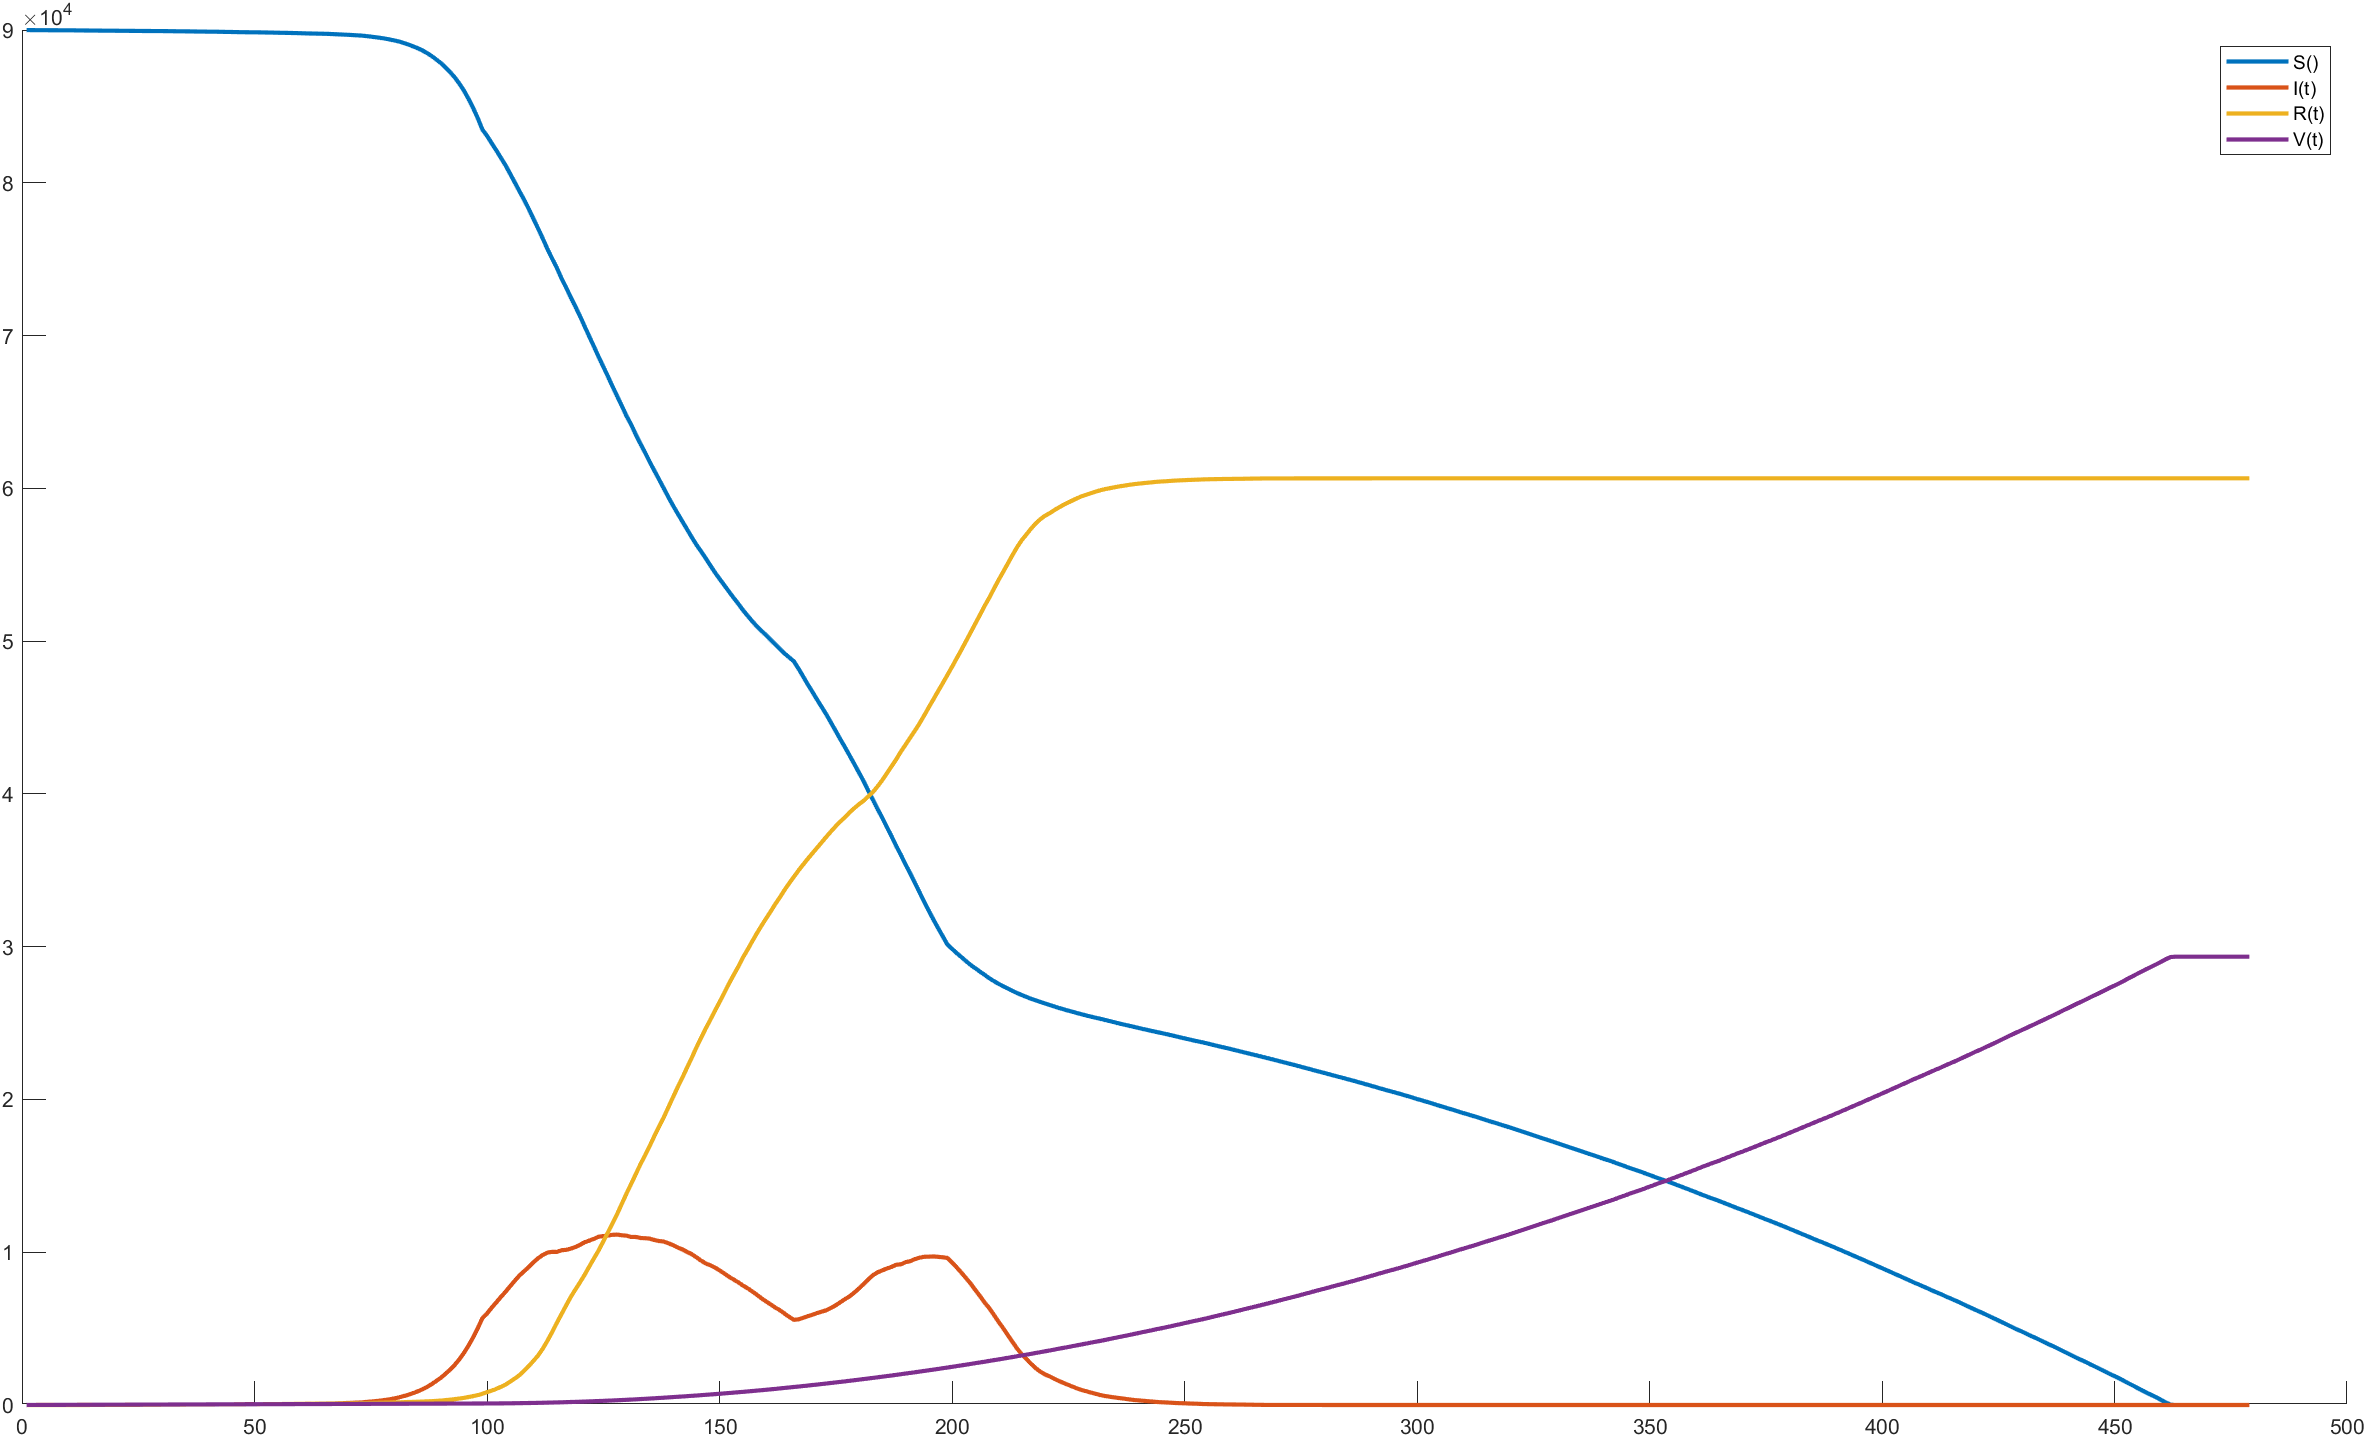
\includegraphics[scale=0.4]{sim1.png}
    \caption{Simulation of COVID-19 using OpenGL, accounting for second wave}
    \label{fig4}
\end{figure}
This graph much more closely matches that of real world data.


\section{Presentation Notes}
I plan on having animations created using MATLAB (and OpenGL for the simulation) that will show the effects of varying the parameters of these differential equations, which I am unable to attach to this paper. The code for many of these samples can by found on my GitHub, which I will attach as a reference here; they will be uploaded by the time of the presentation.



\nocite{*}



\printbibliography

% \subfile{bib.tex}
\end{document}
